\documentclass{article}

\usepackage{pandekten}
\usepackage{dashrule}

\makeatletter
\newcommand*{\shifttext}[1]{%
  \settowidth{\@tempdima}{#1}%
  \hspace{-\@tempdima}#1%
}
\newcommand{\plabel}[1]{%
\shifttext{\textbf{#1}\quad}%
}
\newcommand{\prule}{%
\begin{center}%
\hdashrule[0.5ex]{.99\linewidth}{1pt}{1pt 2.5pt}%
\end{center}%
}

\makeatother

\newcommand{\minusbaseline}{\abovedisplayskip=0pt\abovedisplayshortskip=0pt~\vspace*{-\baselineskip}}%

\setlength{\parindent}{0pt}

\title{Assignment 1}
\author{Ze Chen}

\begin{document}

\maketitle

\plabel{1 (a)}%
The eigenvalues of $T$ are given by
\begin{align*}
    t_1 &= e^{K } \cosh (h) + e^{-K}\sqrt{1+e^{4K}\sinh^2(h)}, \\
    t_2 &= e^{K } \cosh (h) - e^{-K}\sqrt{1+e^{4K}\sinh^2(h)}.
\end{align*}
Therefore,
\[ Z = \Tr(T^N) = t_1^N + t_2^N. \]

\plabel{(b)}%
$-\beta F = \log Z = -N \log t_2$ and therefore
\[ f = \frac{F}{N} = k_B T \log t_2. \]

\plabel{(c)}%
Note that $h = \beta B$.
\begin{align*}
    M &= -\pdv{f}{B} = -\pdv{\log t_2}{h} = \frac{e^{2K} \sinh (h)}{\sqrt{1+e^{4K}\sinh^2(h)}}, \\
    \chi &= \beta \pdv{M}{h} = \frac{\beta e^{2K } \cosh (h)}{\qty[1+e^{4K}\sinh^2(h) ]^{3/2}}.
\end{align*}

The plots against $h$ are given (approximately) below.

\begin{center}
    \begin{tikzpicture}
        \begin{axis}[domain=-1:1,samples=100,xlabel=$h$,ylabel=$M$,axis lines=center, no markers]
            \addplot[color=black] {tanh(5*x)};
        \end{axis}
    \end{tikzpicture}
\end{center}

\begin{center}
    \begin{tikzpicture}
        \begin{axis}[domain=-1:1,samples=100,xlabel=$h$,ylabel=$\chi$,axis lines=center, no markers]
            \addplot[color=black] {7*1/cosh(11*x)};
        \end{axis}
    \end{tikzpicture}
\end{center}

As $K\rightarrow \infty$, the transition of $M$ from $-1$ to $1$ becomes sharp, and the peak of $\chi$ also becomes sharp and divergent.

\plabel{(d)}%
If $T$ is diagonalized as
\[ T = U \begin{pmatrix}
    t_1 & \\ & t_2
\end{pmatrix} U^\dagger,\quad U = \begin{pmatrix}
    u_1 & u_2
\end{pmatrix} \]
where $u_1$ and $u_2$ are (column) eigenvectors,
then
\begin{align*}
    \langle S_i \rangle &= \frac{1}{Z}\Tr[T^N \sigma_z] = \frac{1}{Z}\Tr[\begin{pmatrix}
        t_1^N \\ & t_2^N
    \end{pmatrix}U^\dagger (-\sigma_z) U].
\end{align*}
In the limit $N\rightarrow \infty$, this is
\[ \langle S_i \rangle = -u_2^\dagger \sigma_z u_2 = \frac{e^{2 K } \sinh (h)}{\sqrt{1+e^{4 K } \sinh ^2(h)}}. \]
Let $n=i-j$, then
\begin{align*}
    \langle S_i S_j \rangle &= \frac{1}{Z}\Tr[T^N \sigma_z] \\
    &= \frac{1}{Z}\Tr[\begin{pmatrix}
        t_1^{N-n} \\ & t_2^{N-n}
    \end{pmatrix}U^\dagger (-\sigma_z) U\begin{pmatrix}
        t_1^{n} \\ & t_2^{n}
    \end{pmatrix}U^\dagger (-\sigma_z) U] \\
    &= 4 \qty(\frac{t_1}{t_2})^n (u_2)_1^2 (u_2)_2^2 + \qty((u_2)_1^2 - (u_2)_2^2)^2.
\end{align*}
Therefore
\begin{align*}
    \langle S_i S_j \rangle - \langle S_i \rangle \langle S_j \rangle &= 4 \qty(\frac{t_1}{t_2})^n (u_2)_1^2 (u_2)_2^2 \\
    &= \qty(\frac{t_1}{t_2})^n \cdot \frac{1}{1+e^{4K}\sinh^2(h)}.
\end{align*}

\prule

\plabel{3 (a)}%
Replacing $S_i S_j \rightarrow S_i M + S_j M - M^2$, we find
\[ -\beta H = -\frac{KN}{2}M^2 + \qty(\frac{JM}{N} + h)\sum_i S_i. \]
Therefore
\[ f = \frac{J}{2}N^2 - k_B T\ln 2 - k_B T \ln \cosh \qty(\beta\qty(\frac{JM}{N} + h)). \]
Mean field is a good approximation bacause each site interacts with all other sites with equal coupling, and therefore the energy on each site is given by the interaction with the average spin.

\plabel{(b)}%
We have the self-consistency equation
\[ M = \tanh\qty(\frac{KM}{N} + h). \]
This is identical to that of the NN Ising model.
Therefore $\beta = 1/2$, $\gamma = 1$, $\delta = 3$.

\plabel{(c)}%
No.
To create a domain wall in this infinite range model, one flips a spin,
and this flip affects all other spins, resulting in an energy increase proportional to $N$.

\prule

\plabel{3 (a,b)}%
We may set $v=1$.
To minimize
\[ V = \frac{t}{2} m^2 + u m^4 + m^6, \]
we find
\begin{itemize}
    \item $u\ge 0$ and $t<0$, or $u<0$ and $t \le u^2/2$,
    \begin{align*}
        L_{\text{min}} &= \frac{1}{54} \left(-\sqrt{2} \sqrt{-\left(3 t-2 u^2\right)^3}-9 t u+4 u^3\right), \\
        \overline{m} &= \frac{1}{6} \left(-2u \pm\sqrt{2} \sqrt{2 u^2-3 t}\right).
    \end{align*}
    \item Otherwise, $L_{\text{min}} = 0$ and $\overline{m} = 0$.
\end{itemize}
When $u<0$, the phase transition across $t=u^2/2$ is first order, since $\overline{m}$ jumps from $0$ to a nonzero value.

\begin{center}
    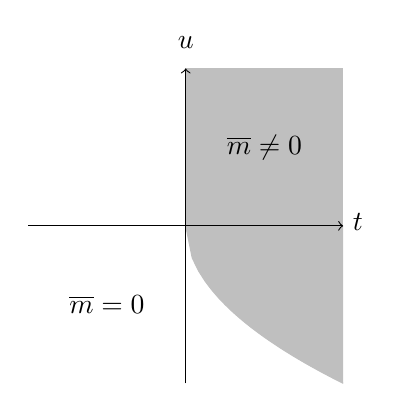
\begin{tikzpicture}
        \draw [domain=0:2,color=lightgray,fill=lightgray,draw=none] plot (\x, -{sqrt(2*\x)}) -- (2,0); 
        \draw [domain=0:2,color=lightgray] plot (\x, -{sqrt(2*\x)});
        \draw [domain=0:2,color=lightgray,fill=lightgray,draw=none] (0,0) -- (0,2) -- (2,2) -- (2,0);
        \draw [->] (0,-2) -- (0,2)                   
            node [label={[above]$u$}] {};
        \draw [->] (-2,0) -- (2,0)           
        node [label={[right,yshift=-0.5ex]$t$}] {};
        \draw (-1,-1) node {$\overline{m} = 0$};
        \draw (1,1) node {$\overline{m} \neq 0$};
    \end{tikzpicture}
\end{center}

\plabel{(c)}%
For $h=0$, the saddle point equation looks like $t m + (?) \cdot m^5 = 0$, and thus $\overline{m} \propto t^{1/4}$, i.e. $\beta = 1/4$.
\par
Taking $h$ into account we find $t m + (?) \cdot m^5 - h = 0$.
Differentiating both sides with respect to $h$ we find
\[ t \chi + (?) \cdot m^4 \chi = 1, \]
and therefore
\[ \chi \sim \frac{1}{t + (?)\cdot m^4} \sim \frac{1}{t}, \]
i.e. $\gamma = 1$.
\par
Setting $t=0$ we find $m^5 \propto h$, i.e. $\delta = 5$.

\prule

\plabel{4}%
For $t<0$, $\vb{m} = \overline{\vb{m}} + \vb*{\phi}$ where $\vb*{\phi} = \vb*{\phi}_\ell + \vb*{\phi}_t$ is the sum of the longitudinal mode and massless Goldstone mode.
Therefore,
\begin{align*}
    Z &\approx \exp[-V\qty(\frac{t}{2}\overline{m}^2 + u\overline{m}^4)] \times \int D\phi_\ell \exp{-\frac{K}{2} \int \dd[d]{x}\qty[(\grad \phi_\ell)^2 + \frac{\mu^2}{K} \phi_\ell^2]} \times \\
    &\phantom{{}\approx{}} \int D\vb*{\phi}_t \exp{-\frac{K}{2} \int \dd[d]{x}\qty[(\grad \phi_t)^2]}.
\end{align*}
The contribution from the Goldstone modes is a overall constant factor to $Z$.
Therefore,
\[ \beta f = \qty(\frac{t}{2}\overline{m}^2 + u\overline{m}^4) + \frac{1}{2} \int \frac{\dd[d]{\vb{q}}}{(2\pi)^d} \ln[K q^2 + \mu^2]. \]
Since $\mu^2 \propto -2(t - t_c)$,
\[ C \propto -\pdv[2]{(\beta f)}{t} = \frac{1}{8u} + 2\int \frac{\dd[d]{\vb{q}}}{(2\pi)^d} \frac{1}{(Kq^2 - 2t)^2}. \]
Therefore
\[ C \sim \frac{1}{8u} + \frac{1}{K^2}\begin{cases}
    \Lambda^{d-4}, & \text{for } d>4,\\
    \xi^{4-d}, & \text{for } d<4.
\end{cases} \]
Similarly important on both sides.
The fluctuation region is given by
\[ \abs{t} < \qty(\frac{1}{\xi_0^d \Delta C})^{\frac{2}{4-d}}. \]

\prule

\plabel{5 (a)}%
Integral on $h_i$ gives an extra factor $\exp(S_i^2 \eta^2/2)$ to $Z$.
Since $S_i^2 = 1$, this is just a constant factor and therefore
\[ F_{\text{annealed}} = F_{\eta = 0} - \frac{1}{2} k_B T N \eta^2, \]
where $F_{\eta = 0}$ was given in problem 2.

\plabel{(b)}%
Now for given configuration $\qty{S_i}_i$,
\begin{align*}
    \langle e^{-\beta H} \rangle_h &= \qty(e^{-\beta H})_{\eta=0} \prod_{i} \exp[\frac{\eta^2}{2}(S_i + S_{i+1})^2] \\
    &= \qty(e^{-\beta H})_{\eta=0} \cdot \qty(\prod_i e^{\eta^2}) \cdot \qty(\prod_i \exp[\eta^2 S_i \cdot S_{i+1}]).
\end{align*}
Effectively,
\[ -\beta H = \frac{K}{2N} \sum_{ij} S_i S_j + \eta^2 \sum_i S_i \cdot S_{i+1}. \]
\par
There may be a phase transition between $K \ll \eta^2$ and $K \gg \eta^2$ since the former is dominated by the NN Ising model and the latter is dominated by the infinite range Ising model.
\par
I don't expect mean field to predict this since mean field does not tell part these two kinds of interactions.

\plabel{(c)}%
For the self-consistency condition to have a nonzero solution, we require $\partial_m$ of RHS be greater than $1$.
\[ K \int P(h) \sech^2(h) \dd{h} > 1. \]
Since $m = g(K m)$ where $g(x) = g_1 x + g_3 x^3 + \cdots$ and $g_1 > 0$, $g_3 < 0$, the behavior near the critical point is not changed.

% \bibliographystyle{plain}
% \bibliography{main}

\end{document}
